\documentclass{article}
\usepackage[margin=0.35in,landscape]{geometry}
\usepackage{tikz}
\usetikzlibrary{calc,shapes.arrows}

\definecolor{etblue}{RGB}{111,152,221}
\definecolor{etpageblue}{RGB}{71,186,227}
\definecolor{etred}{RGB}{226,102,102}
\definecolor{etline}{RGB}{70,70,70}

\tikzset{
  etstate/.style={
    draw=etline,
    line width=0.45pt,
    fill=etblue,
    rectangle,
    minimum width=3.40cm,
    minimum height=0.82cm,
    text width=2.85cm,
    inner xsep=4pt,
    inner ysep=3pt,
    align=center,
    font=\footnotesize,
    text height=1.5ex,
    text depth=.25ex
  },
  etconsequence/.style={
    draw=etline,
    line width=0.45pt,
    fill=etred,
    rectangle,
    minimum width=3.40cm,
    minimum height=0.82cm,
    text width=2.85cm,
    inner xsep=4pt,
    inner ysep=3pt,
    align=center,
    font=\footnotesize,
    text height=1.5ex,
    text depth=.25ex
  },
  etpage/.style={
    draw=etline,
    line width=0.45pt,
    fill=etpageblue,
    single arrow,
    single arrow head extend=0.52cm,
    minimum width=3.40cm,
    minimum height=0.82cm,
    text width=2.20cm,
    inner xsep=4pt,
    inner ysep=3pt,
    align=center,
    font=\footnotesize,
    text height=1.5ex,
    text depth=.25ex
  },
  etlabel/.style={
    font=\scriptsize,
    fill=white,
    inner sep=1pt,
    text=black
  },
  etedge/.style={
    draw=etline,
    line width=0.42pt
  },
  etterminal/.style={
    draw=etline,
    dotted,
    line width=0.42pt
  }
}

\pagestyle{empty}

\begin{document}
\thispagestyle{empty}
\centering
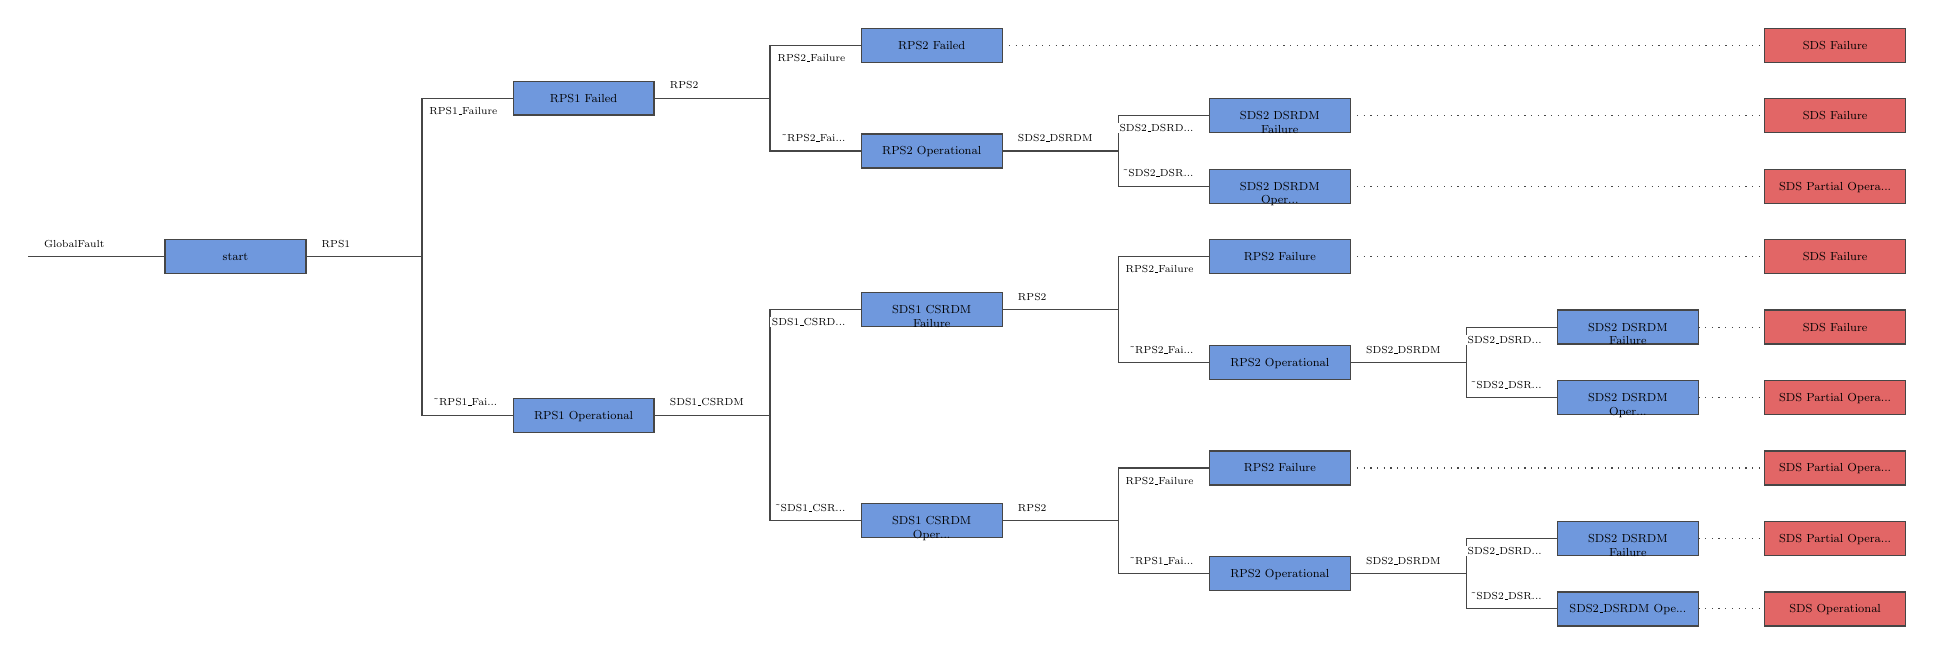
\begin{tikzpicture}[x=1cm,y=1cm,scale=0.5263,transform shape]
\draw[etedge] (6.700, -5.100) -- (8.400, -5.100);
\draw[etedge] (8.400, -5.100) -- (9.500, -5.100) -- (9.500, -1.275) -- (11.700, -1.275);
\draw[etedge] (8.400, -5.100) -- (9.500, -5.100) -- (9.500, -8.925) -- (11.700, -8.925);
\draw[etedge] (15.100, -1.275) -- (16.800, -1.275);
\draw[etedge] (16.800, -1.275) -- (17.900, -1.275) -- (17.900, 0.000) -- (20.100, 0.000);
\draw[etedge] (16.800, -1.275) -- (17.900, -1.275) -- (17.900, -2.550) -- (20.100, -2.550);
\draw[etterminal] (23.500, 0.000) -- (41.900, 0.000);
\draw[etedge] (23.500, -2.550) -- (25.200, -2.550);
\draw[etedge] (25.200, -2.550) -- (26.300, -2.550) -- (26.300, -1.700) -- (28.500, -1.700);
\draw[etedge] (25.200, -2.550) -- (26.300, -2.550) -- (26.300, -3.400) -- (28.500, -3.400);
\draw[etterminal] (31.900, -1.700) -- (41.900, -1.700);
\draw[etterminal] (31.900, -3.400) -- (41.900, -3.400);
\draw[etedge] (15.100, -8.925) -- (16.800, -8.925);
\draw[etedge] (16.800, -8.925) -- (17.900, -8.925) -- (17.900, -6.375) -- (20.100, -6.375);
\draw[etedge] (16.800, -8.925) -- (17.900, -8.925) -- (17.900, -11.475) -- (20.100, -11.475);
\draw[etedge] (23.500, -6.375) -- (25.200, -6.375);
\draw[etedge] (25.200, -6.375) -- (26.300, -6.375) -- (26.300, -5.100) -- (28.500, -5.100);
\draw[etedge] (25.200, -6.375) -- (26.300, -6.375) -- (26.300, -7.650) -- (28.500, -7.650);
\draw[etterminal] (31.900, -5.100) -- (41.900, -5.100);
\draw[etedge] (31.900, -7.650) -- (33.600, -7.650);
\draw[etedge] (33.600, -7.650) -- (34.700, -7.650) -- (34.700, -6.800) -- (36.900, -6.800);
\draw[etedge] (33.600, -7.650) -- (34.700, -7.650) -- (34.700, -8.500) -- (36.900, -8.500);
\draw[etterminal] (40.300, -6.800) -- (41.900, -6.800);
\draw[etterminal] (40.300, -8.500) -- (41.900, -8.500);
\draw[etedge] (23.500, -11.475) -- (25.200, -11.475);
\draw[etedge] (25.200, -11.475) -- (26.300, -11.475) -- (26.300, -10.200) -- (28.500, -10.200);
\draw[etedge] (25.200, -11.475) -- (26.300, -11.475) -- (26.300, -12.750) -- (28.500, -12.750);
\draw[etterminal] (31.900, -10.200) -- (41.900, -10.200);
\draw[etedge] (31.900, -12.750) -- (33.600, -12.750);
\draw[etedge] (33.600, -12.750) -- (34.700, -12.750) -- (34.700, -11.900) -- (36.900, -11.900);
\draw[etedge] (33.600, -12.750) -- (34.700, -12.750) -- (34.700, -13.600) -- (36.900, -13.600);
\draw[etterminal] (40.300, -11.900) -- (41.900, -11.900);
\draw[etterminal] (40.300, -13.600) -- (41.900, -13.600);
\draw[etedge] (0.000, -5.100) -- (3.300, -5.100);
\node[etlabel, anchor=south west] at (7.040, -4.920) {RPS1};
\node[etlabel, anchor=north east] at (11.360, -1.455) {RPS1\_Failure};
\node[etlabel, anchor=south east] at (11.360, -8.745) {\textasciitilde{}RPS1\_Fai...};
\node[etlabel, anchor=south west] at (15.440, -1.095) {RPS2};
\node[etlabel, anchor=north east] at (19.760, -0.180) {RPS2\_Failure};
\node[etlabel, anchor=south east] at (19.760, -2.370) {\textasciitilde{}RPS2\_Fai...};
\node[etlabel, anchor=south west] at (23.840, -2.370) {SDS2\_DSRDM};
\node[etlabel, anchor=north east] at (28.160, -1.880) {SDS2\_DSRD...};
\node[etlabel, anchor=south east] at (28.160, -3.220) {\textasciitilde{}SDS2\_DSR...};
\node[etlabel, anchor=south west] at (15.440, -8.745) {SDS1\_CSRDM};
\node[etlabel, anchor=north east] at (19.760, -6.555) {SDS1\_CSRD...};
\node[etlabel, anchor=south east] at (19.760, -11.295) {\textasciitilde{}SDS1\_CSR...};
\node[etlabel, anchor=south west] at (23.840, -6.195) {RPS2};
\node[etlabel, anchor=north east] at (28.160, -5.280) {RPS2\_Failure};
\node[etlabel, anchor=south east] at (28.160, -7.470) {\textasciitilde{}RPS2\_Fai...};
\node[etlabel, anchor=south west] at (32.240, -7.470) {SDS2\_DSRDM};
\node[etlabel, anchor=north east] at (36.560, -6.980) {SDS2\_DSRD...};
\node[etlabel, anchor=south east] at (36.560, -8.320) {\textasciitilde{}SDS2\_DSR...};
\node[etlabel, anchor=south west] at (23.840, -11.295) {RPS2};
\node[etlabel, anchor=north east] at (28.160, -10.380) {RPS2\_Failure};
\node[etlabel, anchor=south east] at (28.160, -12.570) {\textasciitilde{}RPS1\_Fai...};
\node[etlabel, anchor=south west] at (32.240, -12.570) {SDS2\_DSRDM};
\node[etlabel, anchor=north east] at (36.560, -12.080) {SDS2\_DSRD...};
\node[etlabel, anchor=south east] at (36.560, -13.420) {\textasciitilde{}SDS2\_DSR...};
\node[etlabel, anchor=south west] at (0.340, -4.920) {GlobalFault};
\node[etstate] (initial_end_node) at (5.000, -5.100) {start};
\node[etstate] (e32d490741da4965bd6e63115d27c7b0) at (13.400, -1.275) {RPS1 Failed};
\node[etstate] (n_7f0360aef50c4b978060aa12e08c33e1) at (21.800, 0.000) {RPS2 Failed};
\node[etconsequence] (n_62356e3e_419a_457f_a30c_c0730408f10c) at (43.600, 0.000) {SDS Failure};
\node[etstate] (d87b7a345e6647d8bfceff9793a65128) at (21.800, -2.550) {RPS2 Operational};
\node[etstate] (f79196e2f04740ecb949454bdcbc6a4c) at (30.200, -1.700) {SDS2 DSRDM Failure};
\node[etconsequence] (n_22b7cbf4_e06e_4adf_b32a_4bbfe39d08e9) at (43.600, -1.700) {SDS Failure};
\node[etstate] (b254c8dee42b4635b0bafe7e8412cc71) at (30.200, -3.400) {SDS2 DSRDM Oper...};
\node[etconsequence] (n_2dd0528d_eef1_4221_a579_16c77147576e) at (43.600, -3.400) {SDS Partial Opera...};
\node[etstate] (cc2d9510fd6049538ecccc00abd7ee39) at (13.400, -8.925) {RPS1 Operational};
\node[etstate] (n_3da949ec34bb43c8bd22ac970bba4948) at (21.800, -6.375) {SDS1 CSRDM Failure};
\node[etstate] (n_032924dedd87414ea6a5b2248dc3d7fa) at (30.200, -5.100) {RPS2 Failure};
\node[etconsequence] (n_524e7dec_11a1_4b12_ad9a_fb68a05bb5d2) at (43.600, -5.100) {SDS Failure};
\node[etstate] (n_2f10af84e7744aa4b9a63ead927c6757) at (30.200, -7.650) {RPS2 Operational};
\node[etstate] (beec25cea5254707ac3c4401b6fb9975) at (38.600, -6.800) {SDS2 DSRDM Failure};
\node[etconsequence] (a51b343e_b349_425c_95cb_b80a386d8f8a) at (43.600, -6.800) {SDS Failure};
\node[etstate] (n_07f3584dab3b44c98229857aadac1a6f) at (38.600, -8.500) {SDS2 DSRDM Oper...};
\node[etconsequence] (n_11250f9a_ee47_4fa8_90aa_08fe2f877d44) at (43.600, -8.500) {SDS Partial Opera...};
\node[etstate] (n_7c5ca304488f46ecb51342544607937c) at (21.800, -11.475) {SDS1 CSRDM Oper...};
\node[etstate] (c947e982a644494694804ceabdce5286) at (30.200, -10.200) {RPS2 Failure};
\node[etconsequence] (n_1c2b01ec_f3b9_45e5_aa8f_7cfd7c58bb0b) at (43.600, -10.200) {SDS Partial Opera...};
\node[etstate] (n_18214c7af77d4dac97fc4bd9fd9c8b1d) at (30.200, -12.750) {RPS2 Operational};
\node[etstate] (f4bc2fff7c174a2697eb18a7242a363f) at (38.600, -11.900) {SDS2 DSRDM Failure};
\node[etconsequence] (bcf8926f_f7b6_4b89_a516_aa4d0e9ebccd) at (43.600, -11.900) {SDS Partial Opera...};
\node[etstate] (n_739d0468b31040b0910e7f0396af1d29) at (38.600, -13.600) {SDS2\_DSRDM Ope...};
\node[etconsequence] (n_1b077b91_efa0_4c6b_875d_6a534ac26246) at (43.600, -13.600) {SDS Operational};
\end{tikzpicture}
\end{document}
